\hypertarget{t__redblack_8c}{
\section{t\_\-redblack.c File Reference}
\label{t__redblack_8c}\index{t_redblack.c@{t\_\-redblack.c}}
}


{\tt \#include $<$assert.h$>$}\par
{\tt \#include $<$stdio.h$>$}\par
{\tt \#include $<$stdlib.h$>$}\par
{\tt \#include $<$string.h$>$}\par
{\tt \#include $<$time.h$>$}\par
{\tt \#include \char`\"{}test-harness.h\char`\"{}}\par
{\tt \#include \char`\"{}dbprim.h\char`\"{}}\par
{\tt \#include \char`\"{}dbprim\_\-int.h\char`\"{}}\par


Include dependency graph for t\_\-redblack.c:\begin{figure}[H]
\begin{center}
\leavevmode
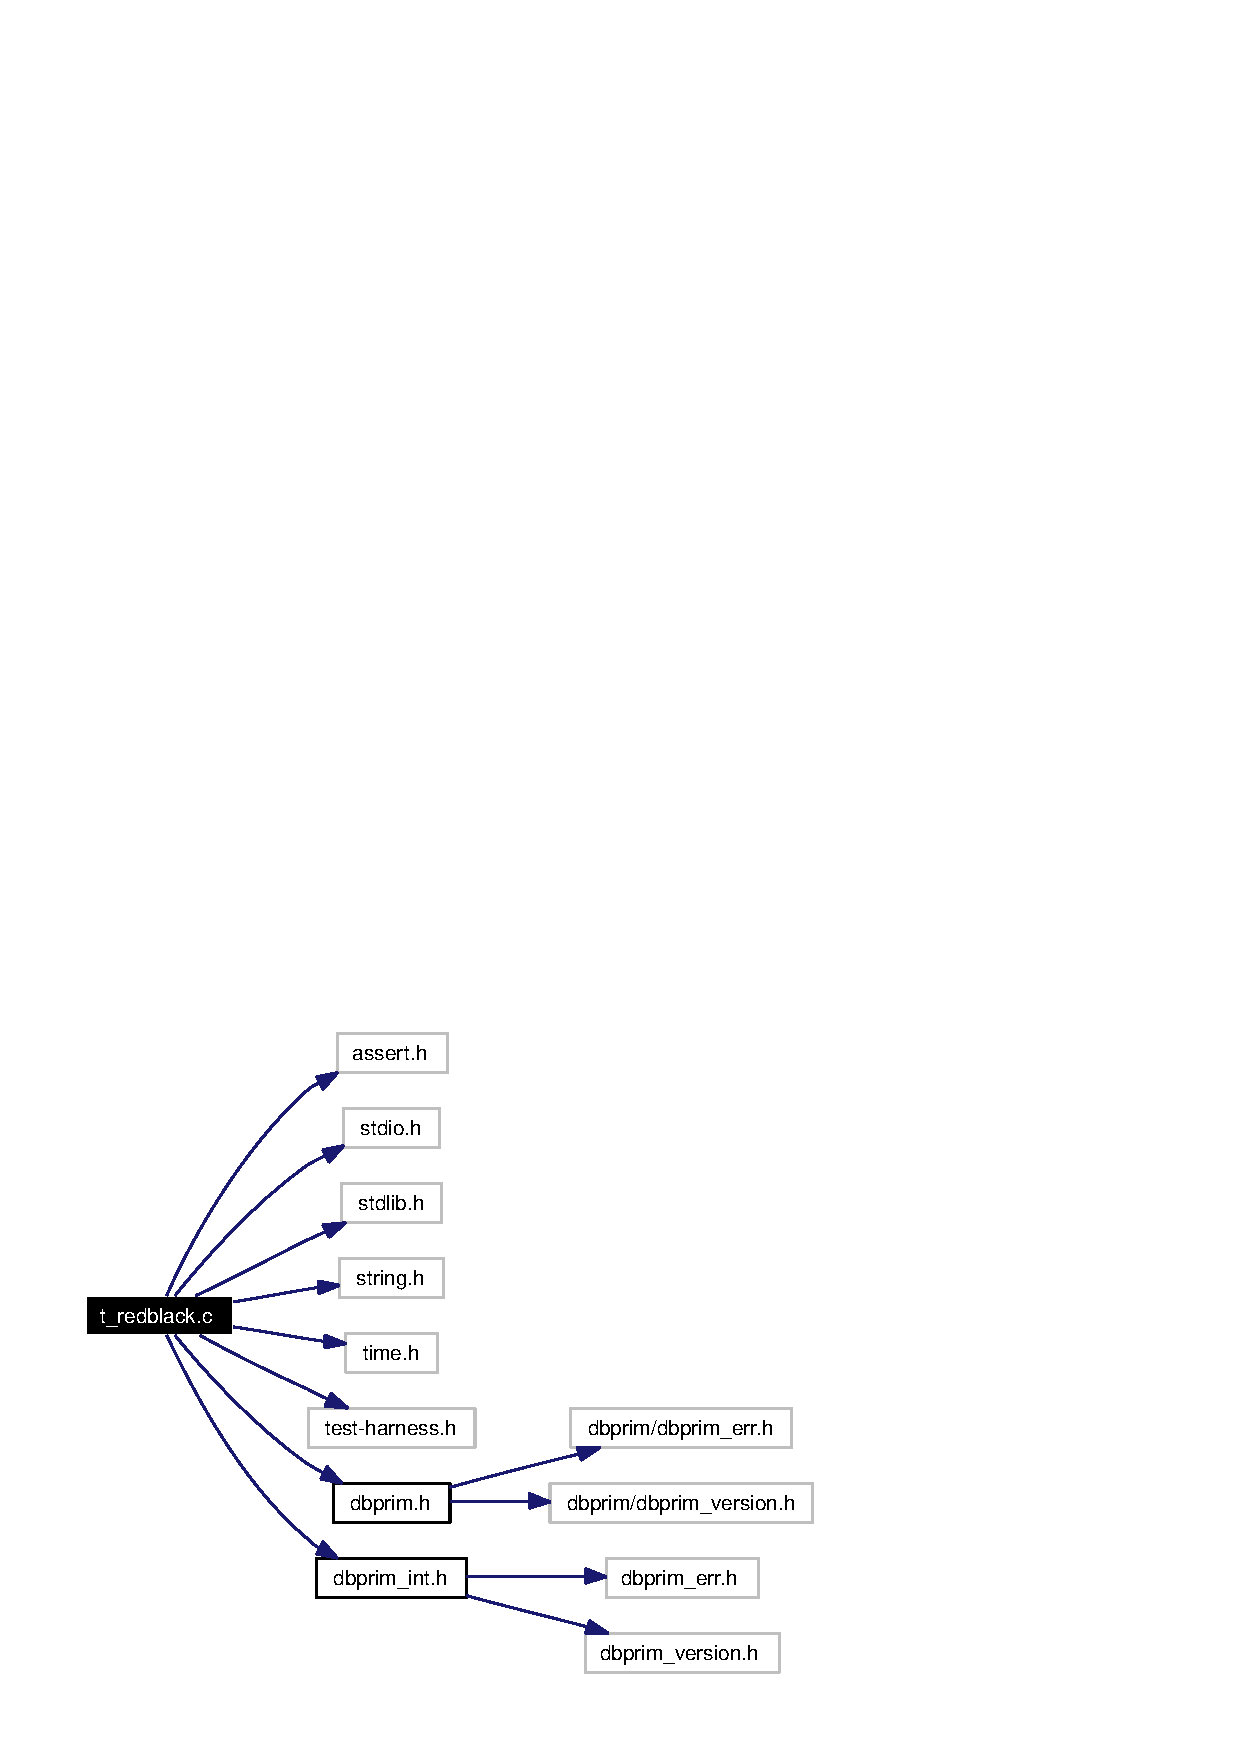
\includegraphics[width=197pt]{t__redblack_8c__incl}
\end{center}
\end{figure}
\subsection*{Data Structures}
\begin{CompactItemize}
\item 
struct \hyperlink{structflush__test}{flush\_\-test}
\item 
struct \hyperlink{structiter__test}{iter\_\-test}
\end{CompactItemize}
\subsection*{Defines}
\begin{CompactItemize}
\item 
\#define \hyperlink{t__redblack_8c_a0}{RBT\_\-ELEM\_\-CNT}
\item 
\#define \hyperlink{t__redblack_8c_a1}{RBT\_\-ELEM\_\-MASK}
\item 
\#define \hyperlink{t__redblack_8c_a2}{selnode}(n, rev)
\item 
\#define \hyperlink{t__redblack_8c_a3}{n\_\-debargs}(node)
\item 
\#define \hyperlink{t__redblack_8c_a4}{STOP\_\-RETURN}
\item 
\#define \hyperlink{t__redblack_8c_a5}{VISIT\_\-RETURN}
\item 
\#define \hyperlink{t__redblack_8c_a6}{ITER\_\-TRIALS}
\end{CompactItemize}
\subsection*{Functions}
\begin{CompactItemize}
\item 
static void \hyperlink{t__redblack_8c_a7}{\_\-make\_\-pre} (\hyperlink{struct__rb__node__s}{rb\_\-node\_\-t} $\ast$node, int $\ast$order, int $\ast$idx, int reverse, unsigned long $\ast$visited)
\item 
static void \hyperlink{t__redblack_8c_a8}{\_\-make\_\-in} (\hyperlink{struct__rb__node__s}{rb\_\-node\_\-t} $\ast$node, int $\ast$order, int $\ast$idx, int reverse, unsigned long $\ast$visited)
\item 
static void \hyperlink{t__redblack_8c_a9}{\_\-make\_\-post} (\hyperlink{struct__rb__node__s}{rb\_\-node\_\-t} $\ast$node, int $\ast$order, int $\ast$idx, int reverse, unsigned long $\ast$visited)
\item 
static void \hyperlink{t__redblack_8c_a10}{make\_\-order} (\hyperlink{struct__rb__tree__s}{rb\_\-tree\_\-t} $\ast$tree, int $\ast$order, unsigned long flags, unsigned long $\ast$visited)
\item 
static int \hyperlink{t__redblack_8c_a11}{comp\_\-order} (int $\ast$o1, int $\ast$o2)
\item 
static int \hyperlink{t__redblack_8c_a12}{treecheck} (\hyperlink{struct__rb__node__s}{rb\_\-node\_\-t} $\ast$node, \hyperlink{struct__rb__node__s}{rb\_\-node\_\-t} $\ast$parent, int bh, int $\ast$tbhp)
\item 
static long \hyperlink{t__redblack_8c_a13}{t\_\-comp} (\hyperlink{struct__rb__tree__s}{rb\_\-tree\_\-t} $\ast$tree, \hyperlink{struct__db__key__s}{db\_\-key\_\-t} $\ast$key1, \hyperlink{struct__db__key__s}{db\_\-key\_\-t} $\ast$key2)
\item 
static unsigned long \hyperlink{t__redblack_8c_a14}{t\_\-flush} (\hyperlink{struct__rb__tree__s}{rb\_\-tree\_\-t} $\ast$tree, \hyperlink{struct__rb__node__s}{rb\_\-node\_\-t} $\ast$node, struct \hyperlink{structflush__test}{flush\_\-test} $\ast$ft)
\item 
static unsigned long \hyperlink{t__redblack_8c_a15}{t\_\-iter} (\hyperlink{struct__rb__tree__s}{rb\_\-tree\_\-t} $\ast$tree, \hyperlink{struct__rb__node__s}{rb\_\-node\_\-t} $\ast$node, struct \hyperlink{structiter__test}{iter\_\-test} $\ast$it)
\item 
int \hyperlink{t__redblack_8c_a16}{main} (int argc, char $\ast$$\ast$argv)
\end{CompactItemize}


\subsection{Define Documentation}
\hypertarget{t__redblack_8c_a6}{
\index{t_redblack.c@{t\_\-redblack.c}!ITER_TRIALS@{ITER\_\-TRIALS}}
\index{ITER_TRIALS@{ITER\_\-TRIALS}!t_redblack.c@{t\_\-redblack.c}}
\subsubsection[ITER\_\-TRIALS]{\setlength{\rightskip}{0pt plus 5cm}\#define ITER\_\-TRIALS}}
\label{t__redblack_8c_a6}




Definition at line 268 of file t\_\-redblack.c.

Referenced by main().\hypertarget{t__redblack_8c_a3}{
\index{t_redblack.c@{t\_\-redblack.c}!n_debargs@{n\_\-debargs}}
\index{n_debargs@{n\_\-debargs}!t_redblack.c@{t\_\-redblack.c}}
\subsubsection[n\_\-debargs]{\setlength{\rightskip}{0pt plus 5cm}\#define n\_\-debargs(node)}}
\label{t__redblack_8c_a3}




Definition at line 134 of file t\_\-redblack.c.

Referenced by treecheck().\hypertarget{t__redblack_8c_a0}{
\index{t_redblack.c@{t\_\-redblack.c}!RBT_ELEM_CNT@{RBT\_\-ELEM\_\-CNT}}
\index{RBT_ELEM_CNT@{RBT\_\-ELEM\_\-CNT}!t_redblack.c@{t\_\-redblack.c}}
\subsubsection[RBT\_\-ELEM\_\-CNT]{\setlength{\rightskip}{0pt plus 5cm}\#define RBT\_\-ELEM\_\-CNT}}
\label{t__redblack_8c_a0}




Definition at line 36 of file t\_\-redblack.c.

Referenced by comp\_\-order(), and main().\hypertarget{t__redblack_8c_a1}{
\index{t_redblack.c@{t\_\-redblack.c}!RBT_ELEM_MASK@{RBT\_\-ELEM\_\-MASK}}
\index{RBT_ELEM_MASK@{RBT\_\-ELEM\_\-MASK}!t_redblack.c@{t\_\-redblack.c}}
\subsubsection[RBT\_\-ELEM\_\-MASK]{\setlength{\rightskip}{0pt plus 5cm}\#define RBT\_\-ELEM\_\-MASK}}
\label{t__redblack_8c_a1}




Definition at line 42 of file t\_\-redblack.c.

Referenced by main().\hypertarget{t__redblack_8c_a2}{
\index{t_redblack.c@{t\_\-redblack.c}!selnode@{selnode}}
\index{selnode@{selnode}!t_redblack.c@{t\_\-redblack.c}}
\subsubsection[selnode]{\setlength{\rightskip}{0pt plus 5cm}\#define selnode(n, rev)}}
\label{t__redblack_8c_a2}




Referenced by \_\-make\_\-in().\hypertarget{t__redblack_8c_a4}{
\index{t_redblack.c@{t\_\-redblack.c}!STOP_RETURN@{STOP\_\-RETURN}}
\index{STOP_RETURN@{STOP\_\-RETURN}!t_redblack.c@{t\_\-redblack.c}}
\subsubsection[STOP\_\-RETURN]{\setlength{\rightskip}{0pt plus 5cm}\#define STOP\_\-RETURN}}
\label{t__redblack_8c_a4}




Definition at line 239 of file t\_\-redblack.c.

Referenced by main(), t\_\-flush(), and t\_\-iter().\hypertarget{t__redblack_8c_a5}{
\index{t_redblack.c@{t\_\-redblack.c}!VISIT_RETURN@{VISIT\_\-RETURN}}
\index{VISIT_RETURN@{VISIT\_\-RETURN}!t_redblack.c@{t\_\-redblack.c}}
\subsubsection[VISIT\_\-RETURN]{\setlength{\rightskip}{0pt plus 5cm}\#define VISIT\_\-RETURN}}
\label{t__redblack_8c_a5}




Definition at line 240 of file t\_\-redblack.c.

Referenced by main(), t\_\-flush(), and t\_\-iter().

\subsection{Function Documentation}
\hypertarget{t__redblack_8c_a8}{
\index{t_redblack.c@{t\_\-redblack.c}!_make_in@{\_\-make\_\-in}}
\index{_make_in@{\_\-make\_\-in}!t_redblack.c@{t\_\-redblack.c}}
\subsubsection[\_\-make\_\-in]{\setlength{\rightskip}{0pt plus 5cm}static void \_\-make\_\-in (\hyperlink{struct__rb__node__s}{rb\_\-node\_\-t} $\ast$ {\em node}, int $\ast$ {\em order}, int $\ast$ {\em idx}, int {\em reverse}, unsigned long $\ast$ {\em visited})\hspace{0.3cm}{\tt  \mbox{[}static\mbox{]}}}}
\label{t__redblack_8c_a8}




Definition at line 62 of file t\_\-redblack.c.

References rn\_\-value, and selnode.

Referenced by make\_\-order().\hypertarget{t__redblack_8c_a9}{
\index{t_redblack.c@{t\_\-redblack.c}!_make_post@{\_\-make\_\-post}}
\index{_make_post@{\_\-make\_\-post}!t_redblack.c@{t\_\-redblack.c}}
\subsubsection[\_\-make\_\-post]{\setlength{\rightskip}{0pt plus 5cm}static void \_\-make\_\-post (\hyperlink{struct__rb__node__s}{rb\_\-node\_\-t} $\ast$ {\em node}, int $\ast$ {\em order}, int $\ast$ {\em idx}, int {\em reverse}, unsigned long $\ast$ {\em visited})\hspace{0.3cm}{\tt  \mbox{[}static\mbox{]}}}}
\label{t__redblack_8c_a9}




Definition at line 77 of file t\_\-redblack.c.

References rn\_\-left, rn\_\-right, and rn\_\-value.

Referenced by make\_\-order().\hypertarget{t__redblack_8c_a7}{
\index{t_redblack.c@{t\_\-redblack.c}!_make_pre@{\_\-make\_\-pre}}
\index{_make_pre@{\_\-make\_\-pre}!t_redblack.c@{t\_\-redblack.c}}
\subsubsection[\_\-make\_\-pre]{\setlength{\rightskip}{0pt plus 5cm}static void \_\-make\_\-pre (\hyperlink{struct__rb__node__s}{rb\_\-node\_\-t} $\ast$ {\em node}, int $\ast$ {\em order}, int $\ast$ {\em idx}, int {\em reverse}, unsigned long $\ast$ {\em visited})\hspace{0.3cm}{\tt  \mbox{[}static\mbox{]}}}}
\label{t__redblack_8c_a7}




Definition at line 46 of file t\_\-redblack.c.

References rn\_\-left, rn\_\-right, and rn\_\-value.

Referenced by make\_\-order().\hypertarget{t__redblack_8c_a11}{
\index{t_redblack.c@{t\_\-redblack.c}!comp_order@{comp\_\-order}}
\index{comp_order@{comp\_\-order}!t_redblack.c@{t\_\-redblack.c}}
\subsubsection[comp\_\-order]{\setlength{\rightskip}{0pt plus 5cm}static int comp\_\-order (int $\ast$ {\em o1}, int $\ast$ {\em o2})\hspace{0.3cm}{\tt  \mbox{[}static\mbox{]}}}}
\label{t__redblack_8c_a11}




Definition at line 116 of file t\_\-redblack.c.

References RBT\_\-ELEM\_\-CNT.

Referenced by main().\hypertarget{t__redblack_8c_a16}{
\index{t_redblack.c@{t\_\-redblack.c}!main@{main}}
\index{main@{main}!t_redblack.c@{t\_\-redblack.c}}
\subsubsection[main]{\setlength{\rightskip}{0pt plus 5cm}int main (int {\em argc}, char $\ast$$\ast$ {\em argv})}}
\label{t__redblack_8c_a16}




Definition at line 293 of file t\_\-redblack.c.

References comp\_\-order(), DB\_\-KEY\_\-INIT, dk\_\-len, iter\_\-test::idx, ITER\_\-TRIALS, iter\_\-test::last\_\-node, make\_\-order(), iter\_\-test::order, RBT\_\-ELEM\_\-CNT, RBT\_\-ELEM\_\-MASK, RBT\_\-ORDER\_\-MASK, rn\_\-init(), rn\_\-key, rt\_\-add(), rt\_\-count, rt\_\-find(), rt\_\-flush(), rt\_\-init(), rt\_\-iter(), rt\_\-next(), rt\_\-remove(), rt\_\-root, iter\_\-test::stop\_\-node, flush\_\-test::stop\_\-node, STOP\_\-RETURN, t\_\-comp(), t\_\-flush(), t\_\-iter(), treecheck(), VISIT\_\-RETURN, iter\_\-test::visited, and flush\_\-test::visited.

Here is the call graph for this function:\begin{figure}[H]
\begin{center}
\leavevmode
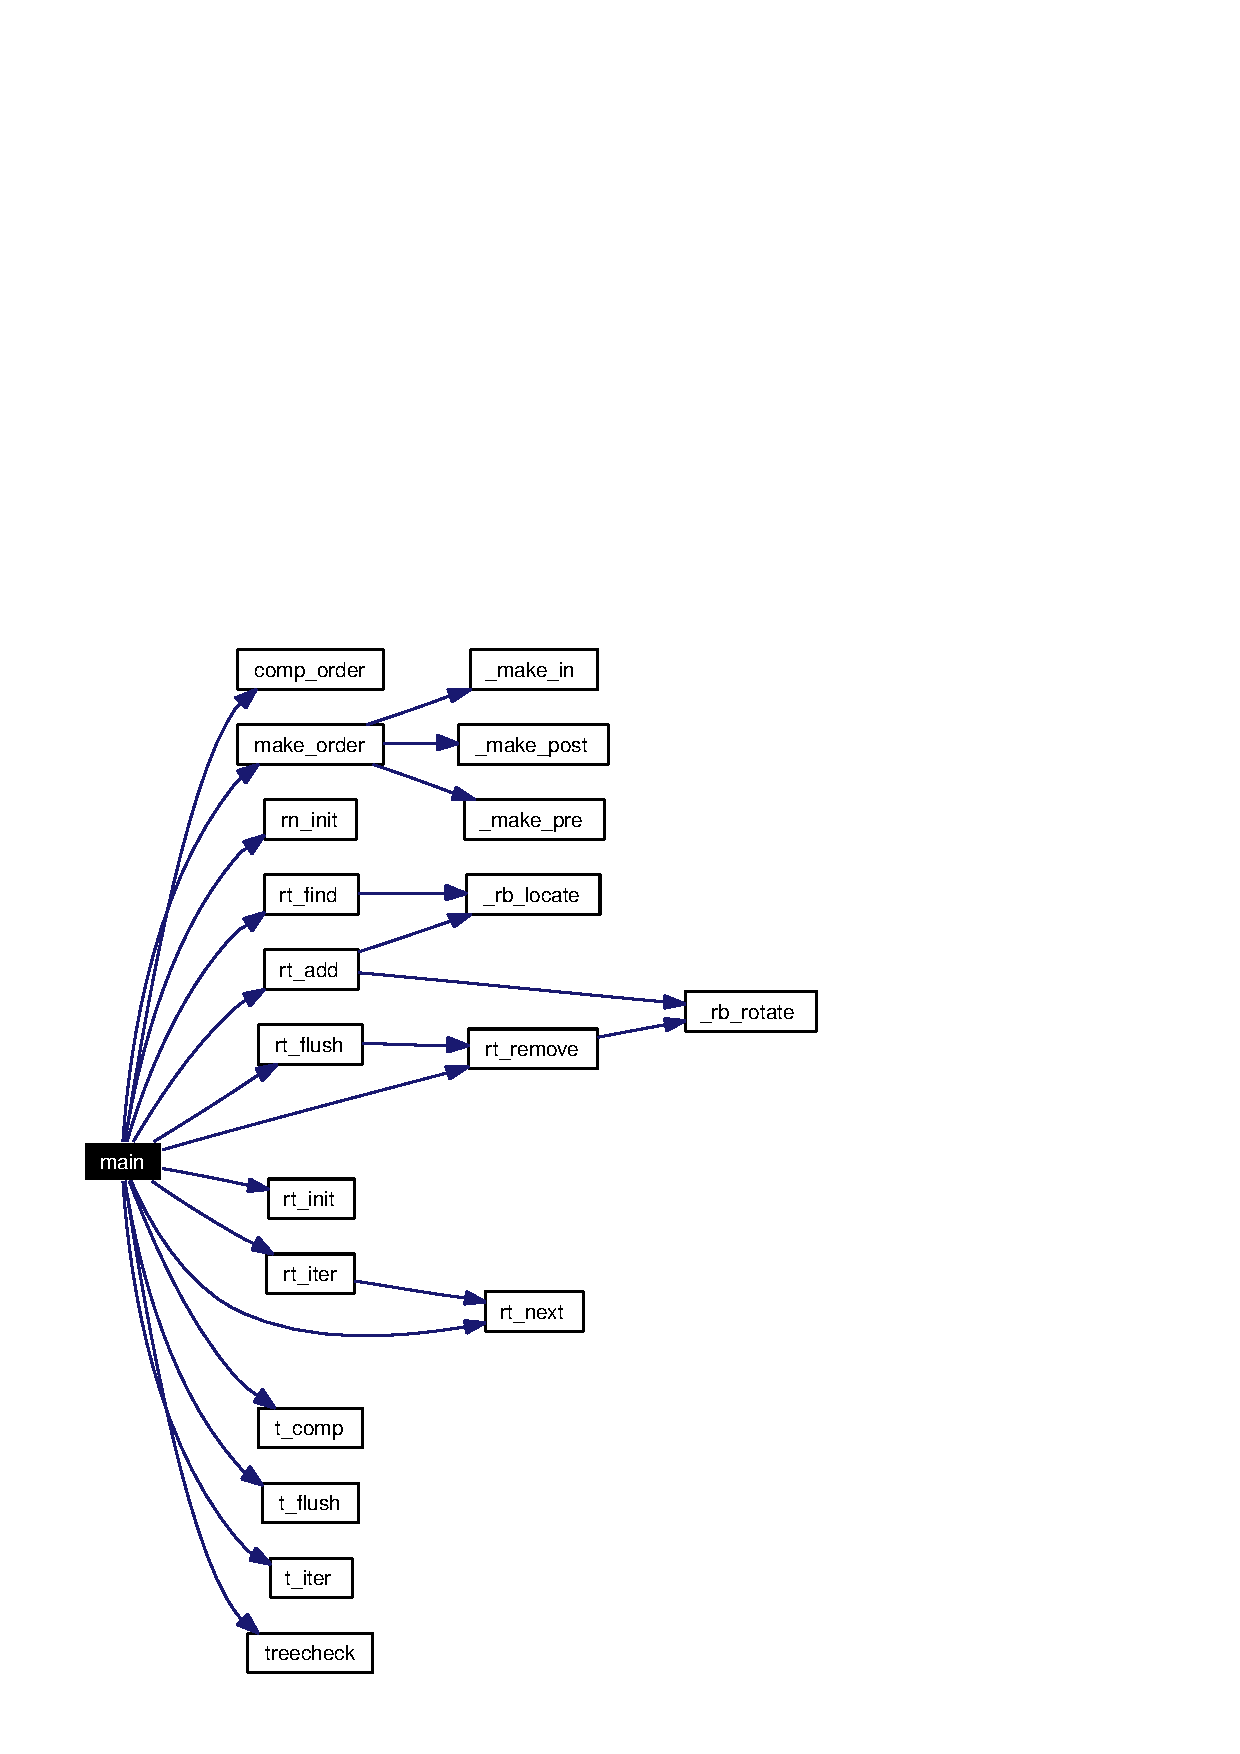
\includegraphics[width=198pt]{t__redblack_8c_a16_cgraph}
\end{center}
\end{figure}
\hypertarget{t__redblack_8c_a10}{
\index{t_redblack.c@{t\_\-redblack.c}!make_order@{make\_\-order}}
\index{make_order@{make\_\-order}!t_redblack.c@{t\_\-redblack.c}}
\subsubsection[make\_\-order]{\setlength{\rightskip}{0pt plus 5cm}static void make\_\-order (\hyperlink{struct__rb__tree__s}{rb\_\-tree\_\-t} $\ast$ {\em tree}, int $\ast$ {\em order}, unsigned long {\em flags}, unsigned long $\ast$ {\em visited})\hspace{0.3cm}{\tt  \mbox{[}static\mbox{]}}}}
\label{t__redblack_8c_a10}




Definition at line 93 of file t\_\-redblack.c.

References \_\-make\_\-in(), \_\-make\_\-post(), \_\-make\_\-pre(), DB\_\-FLAG\_\-REVERSE, RBT\_\-ORDER\_\-IN, RBT\_\-ORDER\_\-POST, RBT\_\-ORDER\_\-PRE, and rt\_\-root.

Referenced by main().

Here is the call graph for this function:\begin{figure}[H]
\begin{center}
\leavevmode
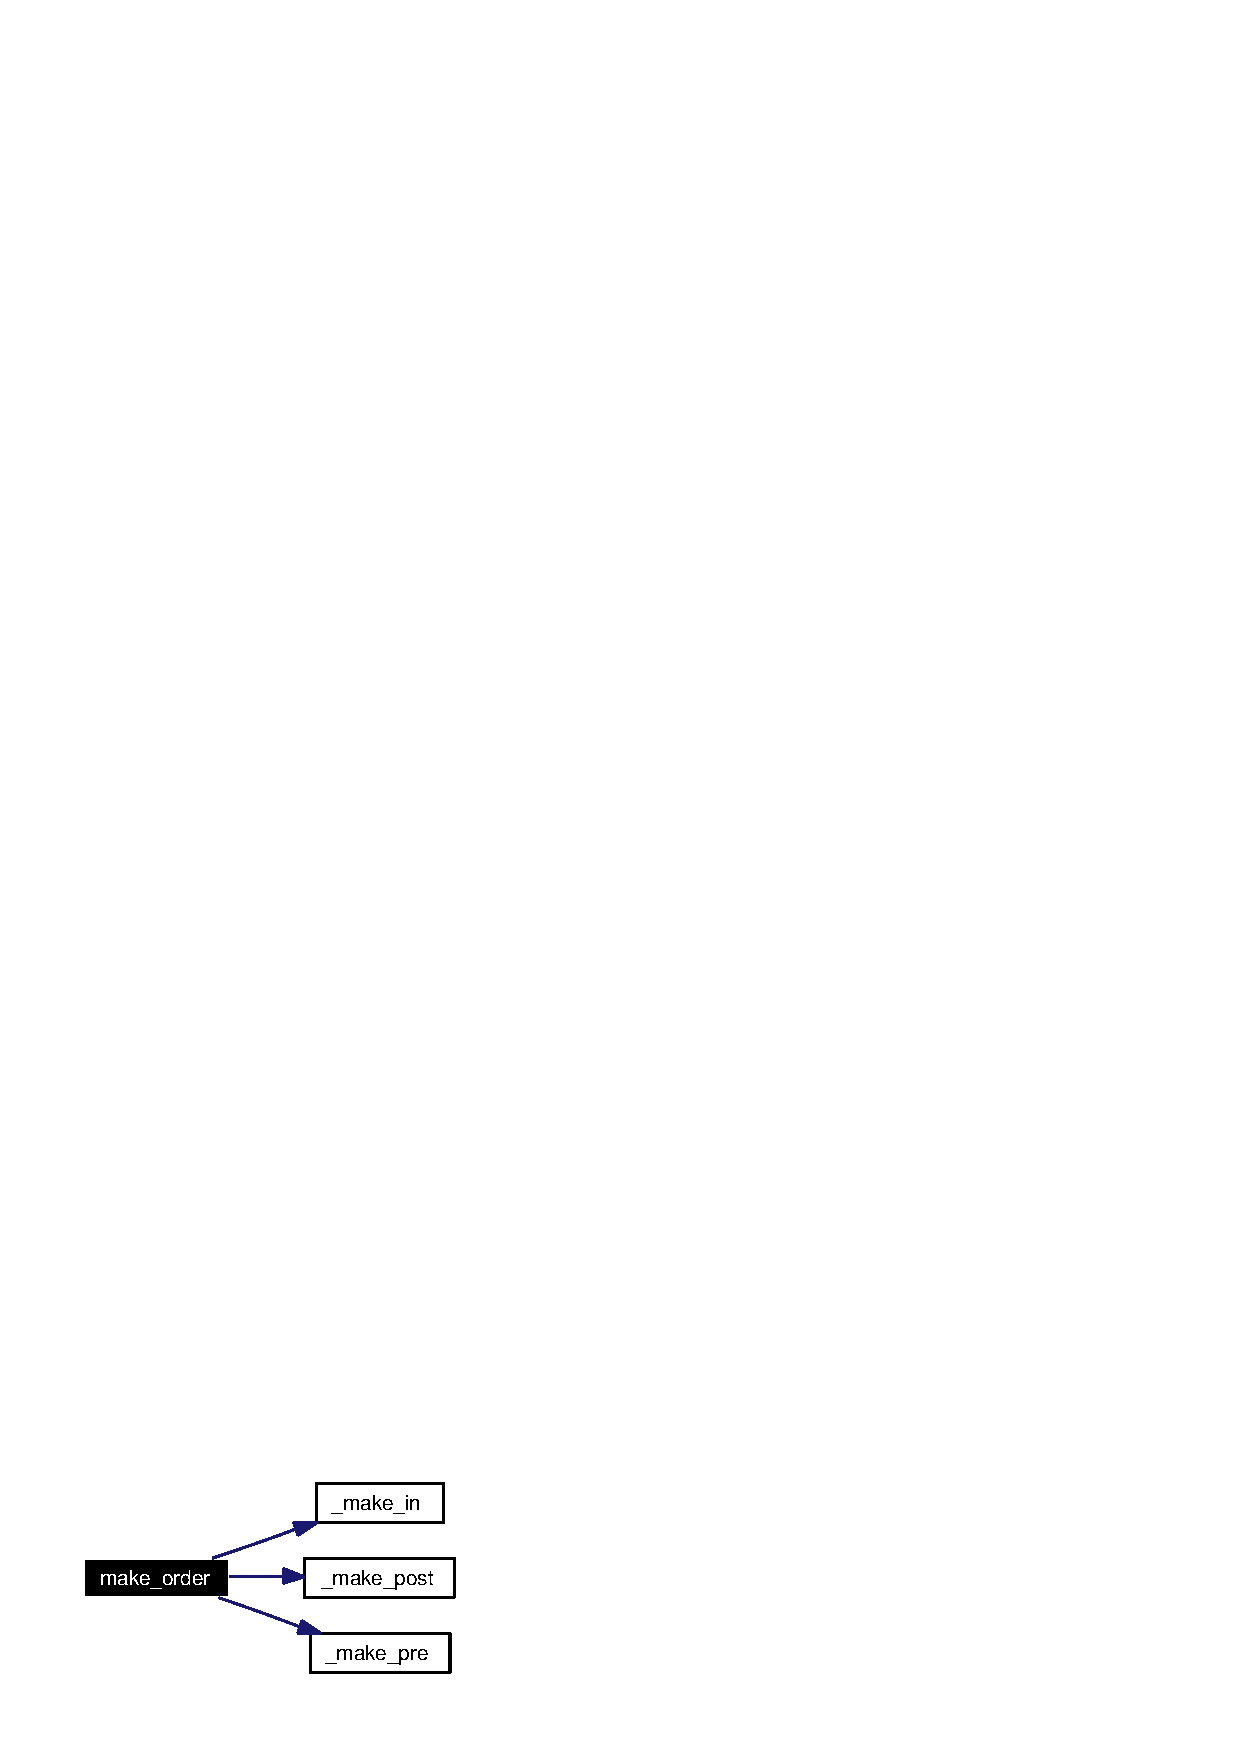
\includegraphics[width=111pt]{t__redblack_8c_a10_cgraph}
\end{center}
\end{figure}
\hypertarget{t__redblack_8c_a13}{
\index{t_redblack.c@{t\_\-redblack.c}!t_comp@{t\_\-comp}}
\index{t_comp@{t\_\-comp}!t_redblack.c@{t\_\-redblack.c}}
\subsubsection[t\_\-comp]{\setlength{\rightskip}{0pt plus 5cm}static long t\_\-comp (\hyperlink{struct__rb__tree__s}{rb\_\-tree\_\-t} $\ast$ {\em tree}, \hyperlink{struct__db__key__s}{db\_\-key\_\-t} $\ast$ {\em key1}, \hyperlink{struct__db__key__s}{db\_\-key\_\-t} $\ast$ {\em key2})\hspace{0.3cm}{\tt  \mbox{[}static\mbox{]}}}}
\label{t__redblack_8c_a13}




Definition at line 228 of file t\_\-redblack.c.

References dk\_\-len.\hypertarget{t__redblack_8c_a14}{
\index{t_redblack.c@{t\_\-redblack.c}!t_flush@{t\_\-flush}}
\index{t_flush@{t\_\-flush}!t_redblack.c@{t\_\-redblack.c}}
\subsubsection[t\_\-flush]{\setlength{\rightskip}{0pt plus 5cm}static unsigned long t\_\-flush (\hyperlink{struct__rb__tree__s}{rb\_\-tree\_\-t} $\ast$ {\em tree}, \hyperlink{struct__rb__node__s}{rb\_\-node\_\-t} $\ast$ {\em node}, struct \hyperlink{structflush__test}{flush\_\-test} $\ast$ {\em ft})\hspace{0.3cm}{\tt  \mbox{[}static\mbox{]}}}}
\label{t__redblack_8c_a14}




Definition at line 244 of file t\_\-redblack.c.

References dk\_\-len, rn\_\-key, flush\_\-test::stop\_\-node, STOP\_\-RETURN, VISIT\_\-RETURN, and flush\_\-test::visited.

Referenced by main().\hypertarget{t__redblack_8c_a15}{
\index{t_redblack.c@{t\_\-redblack.c}!t_iter@{t\_\-iter}}
\index{t_iter@{t\_\-iter}!t_redblack.c@{t\_\-redblack.c}}
\subsubsection[t\_\-iter]{\setlength{\rightskip}{0pt plus 5cm}static unsigned long t\_\-iter (\hyperlink{struct__rb__tree__s}{rb\_\-tree\_\-t} $\ast$ {\em tree}, \hyperlink{struct__rb__node__s}{rb\_\-node\_\-t} $\ast$ {\em node}, struct \hyperlink{structiter__test}{iter\_\-test} $\ast$ {\em it})\hspace{0.3cm}{\tt  \mbox{[}static\mbox{]}}}}
\label{t__redblack_8c_a15}




Definition at line 272 of file t\_\-redblack.c.

References dk\_\-len, iter\_\-test::idx, iter\_\-test::last\_\-node, iter\_\-test::order, rn\_\-key, iter\_\-test::stop\_\-node, STOP\_\-RETURN, VISIT\_\-RETURN, and iter\_\-test::visited.\hypertarget{t__redblack_8c_a12}{
\index{t_redblack.c@{t\_\-redblack.c}!treecheck@{treecheck}}
\index{treecheck@{treecheck}!t_redblack.c@{t\_\-redblack.c}}
\subsubsection[treecheck]{\setlength{\rightskip}{0pt plus 5cm}static int treecheck (\hyperlink{struct__rb__node__s}{rb\_\-node\_\-t} $\ast$ {\em node}, \hyperlink{struct__rb__node__s}{rb\_\-node\_\-t} $\ast$ {\em parent}, int {\em bh}, int $\ast$ {\em tbhp})\hspace{0.3cm}{\tt  \mbox{[}static\mbox{]}}}}
\label{t__redblack_8c_a12}




Definition at line 140 of file t\_\-redblack.c.

References dk\_\-len, n\_\-debargs, rn\_\-isblack, rn\_\-isred, rn\_\-key, \_\-rb\_\-node\_\-s::rn\_\-left, \_\-rb\_\-node\_\-s::rn\_\-parent, and \_\-rb\_\-node\_\-s::rn\_\-right.

Referenced by main().